\chapter{Appendix: Forward Error Correction}
\label{appFEC}
\section{Hamming Code}

Hamming Code/Decode algorithm 

In a Hamming code parity-check bits are added to the original message bits. Any bit, whether the bits of the origninal messege or the parity-check bits, 
would have a unique combination of check-bits associated with it. The original-bits and the parity-check bits are spoted at particular locations in
the frame, the pattern is followed in any Hamming Code and no matter how many check-bits are included. The parity bit $c_i$ is used to convey the parity 
bit for all bits in the code whose position have a binary representation with a $1$ in position $i$. The Table ~ref{tab:HAMING} presents 

\begin{table}[!ht]
        \begin{center}
                \begin{tabular}{|c c|c|c|c|c|c|c|c|c|c|c|c|c|c|c|c|c|}
\hline
Bit Position & & 1 & 2 & 3 & 4 & 5 & 6 & 7 & 8 & 9 & 10 & 11 & 12 & 13 & 14 & 15 & 16  \\ \hline
%Encoded data Bit 

\multicolumn{2}{|c|}{Encoded data Bit } & \colorbox{green}{p1}	& \colorbox{green}{p2} &	d1 &	\colorbox{green}{p4}	& d2 &	d3 &	d4 &	\colorbox{green}{p8} &	d5 & d6 &	d7 &	d8 &	d9 &	d10 &	d11 &	\colorbox{green}{p16}  \\ \hline

\multirow{5}{*}{Paritiy Bit} 
		 & \multicolumn{1}{|c|}{\colorbox{green}{p1}} & X &  & X &  & X &  & X &  & X &  &X &  &X&  &X &  \\ \cline{2-18}%
		 & \multicolumn{1}{|c|}{\colorbox{green}{p2}} & & X &X & & & X& X& & &X &X & & &X &X &  \\  \cline{2-18}%
		 & \multicolumn{1}{|c|}{\colorbox{green}{p4}} & & & &X &X &X &X & & & & &X &X &X &X &   \\  \cline{2-18}%
		 & \multicolumn{1}{|c|}{\colorbox{green}{p8}} & & & & & & & &X &X &X &X &X &X &X &X &   \\  \cline{2-18}%
		 & \multicolumn{1}{|c|}{\colorbox{green}{p16}} & & & & & & & & & & & & & &  & & X  \\ \hline

        	\end{tabular}
          \caption{Postion of the parity-check bits and Information bits in a Hamming Code}
	  \label{tab:HAMING}
	\end{center} 
\end{table}

The parity bits are calculate as follows:

\begin{table}[!ht]
        \begin{center}
                \begin{tabular}{c c c c c c c c c c c c c c c c c}
	         p1= & d1 &$\oplus$& d2 &$\oplus$&    &$\oplus$& d4 &$\oplus$& d5 &          &    &$\oplus$& d7 &          &     \\
		 p2= & d1 &        &    &$\oplus$& d3 &$\oplus$& d4 &$\oplus$&    & $\oplus$ & d6 &$\oplus$& d7 &          &      \\
	         p4= &    &        &    &        &    &        &    &$\oplus$& d5 & $\oplus$ & d6 &$\oplus$& d7 & $\oplus$ & d8   \\
... = & .... &&&&&&&&&&& \\
	
		 		\end{tabular}   
	\end{center}
\end{table}

The decoding process will calculate the parity-check bits again 

\begin{table}[!ht]
        \begin{center}
                \begin{tabular}{c c c c c c c c c c c c c c c c c}
	         p1'= & d1 &$\oplus$& d2 &$\oplus$&    &$\oplus$& d4 &$\oplus$& d5 &          &    &$\oplus$& d7 &          &     \\
		 p2'= & d1 &        &    &$\oplus$& d3 &$\oplus$& d4 &$\oplus$&    & $\oplus$ & d6 &$\oplus$& d7 &          &      \\
	         p4'= &    &        &    &        &    &        &    &$\oplus$& d5 & $\oplus$ & d6 &$\oplus$& d7 & $\oplus$ & d8   \\
... = & .... &&&&&&&&&&& \\
	
		 		\end{tabular}   
	\end{center}
\end{table}

The exclusive-or operation between the received parity-check  bits: p1,p2 etc.. and the calculate parity-check  bits: p1',p2' etc... 

\begin{table}[!ht]
        \begin{center}
                \begin{tabular}{cccc}
         e1 = & p1 &$\oplus$& p1' \\
				 e2 = & p2 &$\oplus$& p2' \\
			   e3 = & p4 &$\oplus$& p4' \\
				... = & ....  &$\oplus$& .... \\
		 		\end{tabular}   
	\end{center}
\end{table}

will indicate no error in the frame if all $e_i$ are 0, otherwise the value indicate the position of error in the frame, and it shall be correct by flipping the received value.


%%%%%%%%%%%%%%%%%%%%%%%%%%%%%%%%%%%%%%%%%%%%%%%%%%%%%%%%%%%%%%%%%%%%%%
\section{Reed Solomon}

Reed Solomon encoding and decoding is based on the domain of Galois  field $GF(2^m)$.  The value, m, is the code word size of the encoding. 
The \ControlMessage is subdivided into code blocks of length $m$ bits and check values must be computed for each code block. 
The frames transmitted consists of \ControlMessage frames and check frames used in reconstructing lost frames. 

The algorithm requires an encoding/decoding matrix of $n+k$ rows and n columns
with following properties:


\begin{itemize}
    \item Identity Matrix Property: the first $n$ rows constitute a $n \times n$ identity matrix, $I$. 
    \item Independent Linearity: any n of the $n+k$ rows are linearly independent. This property ensures that any collection of exactly $n$ rows constitutes an invertible $n \times $ matrix.

The required matrix for encoding is derived from Vandermonde matrix. For arbitrary n and m, this matrix has the following form. The fact
that the largest value in $GF(2^m)$ is $2^m-1$ necessarily constrains the number of rows and columns in the matrix $(n + k)$ to be less than or equal to $2^m$
\end{itemize}

\vspace{0.5cm}
\begin{center}
$V= 
\begin{bmatrix} 

0^0 & 0^1 & 0^2 & .... & 0^{(n-1)} \\ 
1^0 & 1^1 & 1^2 & .... & 1^{(n-1)} \\
2^0 & 2^1 & 2^2 & .... & 2^{(n-1)} \\ 
... & ... & ... & .....& ...	   \\
(2^m-1)^0 & (2^m-1)^1 & (2^m-1)^2 & .... & (2^m-1)^{(n-1)} \\

\end{bmatrix}$
\end{center}
\vspace{0.5cm}

This matrix $V$ doesn't possess property of idependant linearity, but clearly
does not possess the identity matrix. Nevertheless, by a series of linear transformations in which a multiple of one
column is added to another, we can obtain a matrix with the identity matrix
property  while preserving the independence of the vectors. We will call this transformed matrix $D$.

\vspace{0.5cm}
\begin{center}
$D= 
\begin{bmatrix} 

1 & 0 & 0 & .... & 0 \\ 
0 & 1 & 0 & .... & 0  \\
0 & 0 & 1 & .... & 0 \\ 
... & ... & ...  & .....& ....\\
0 & 0 & 0 & .... & 1\\ 
a & b & c & .... & d \\
a_1 & b_1 & c_1 & .... & d_1 \\
a_2 & b_2 & c_2 & .... & d_2 \\
a_3 & b_3 & c_3 & .... & d_3 \\
... & ... & ...  & .....& ....\\
a_{n-1} & b_{n-1} & c_{n-1} & .... & d_{n-1} \\

\end{bmatrix}$
\end{center}
\vspace{0.5cm}


The bottom $k$ rows of the transformed Vandermonde matrix, $D$, constitute the encoding matrix $E$ that is used to create the $k$ check frames. The matrix $E$ has dimension $k \times n$ where $k$ is the number of check frames and $n$ is the number of \ControlMessage frames. When the $n \times 1$ vector of code block is multiplied by $E$ the check values is produced. The encoding algorithm each code word is $b$ bits. If an actual \ControlMessage consisted of 4000 $b$ bits, the process described above would have to be repeated 4000 times, once for each code block in the \ControlMessage.
\vspace{0.5cm}

\begin{center}
$E= 
\begin{bmatrix} 
a   & b   & c   & ... & d		\\
a_1 & b_1 & c_1 & ... & d_1 \\
a_2 & b_2 & c_2 & ... & d_2 \\
a_3 & b_3 & c_3 & ... & d_3 \\
... & ... & ... & ... & ...\\
a_{n-1} & b_{n-1} & c_{n-1} & ... & d_{n-1}
\end{bmatrix}$
\end{center}

\vspace{0.5cm}

\begin{center}
$
\begin{bmatrix} 
a   & b   & c   & ... & d   \\
a_1 & b_1 & c_1 & ... & d_1 \\
a_2 & b_2 & c_2 & ... & d_2 \\
a_3 & b_3 & c_3 & ... & d_3 \\
... & ... & ... & ... & ... \\
a_{n-1} & b_{n-1} & c_{n-1} & ... & d_{n-1} 
\end{bmatrix}
$
$\times$
$
\begin{bmatrix} 
bit \\ bit_1 \\ bit_2 \\ bit_3 \\...\\bit_{n-1} 
\end{bmatrix} 
$
$=$
$
\begin{bmatrix} 
ebit \\ ebit_1 \\ ebit_2 \\ ebit_3 \\ ... \\ ebit_{n-1} 
\end{bmatrix}
$
\end{center}

\vspace{0.5cm}

The decoding algorithm supposes a collection of n frames including both \ControlMessage  and check frames have been received. 
We extract the n rows of the matrix corresponding the $n$ received packets. We call this $n \times n$ matrix $D'$. We invert $D'$ to obtain $D'^{-1}$.
Then the product of $D'^{-1}$ and the received mixture of data words and check words recovers the data words $d0, ...d_{n-1}$.

\begin{center}
$D'=
\begin{bmatrix} 
a   & b   & c   & ... & d   \\
a_1 & b_1 & c_1 & ... & d_1 \\
a_3 & b_3 & c_3 & ... & d_3 \\
... & ... & ... & ... & ... \\
a_{n-1} & b_{n-1} & c_{n-1} & ... & d_{n-1} 
\end{bmatrix}
$
\end{center}
\vspace{0.5cm}

\begin{center}
$
\begin{bmatrix} 
a   & b   & c   & ... & d   \\
a_1 & b_1 & c_1 & ... & d_1 \\
a_3 & b_3 & c_3 & ... & d_3 \\
... & ... & ... & ... & ... \\
a_{n-1} & b_{n-1} & c_{n-1} & ... & d_{n-1} 
\end{bmatrix}
$
$\times$
$
\begin{bmatrix} 
ebit \\ ebit_1  \\ ebit_3 \\ ... \\ ebit_{n-1} 
\end{bmatrix}
$
$=$
$
\begin{bmatrix} 
a \\ b \\ c \\ ... \\ z 
\end{bmatrix}
$
\end{center}
\vspace{0.5cm}
Because the receiver also knows the algorithm by which the check frames were constructed, inverting $D'$ yields $D'^{-1}$. Multiplying the received check values by $D'{-1}$ recovers the original values.

\begin{center}
$D'^{-1}$ 
$\times$
$
\begin{bmatrix} 
a \\ b \\ c \\ ... \\ z 
\end{bmatrix}
$
$=$
$
\begin{bmatrix} 
bit \\ bit_1 \\ bit_2 \\ bit_3 \\...\\bit_{n-1} 
\end{bmatrix} 
$
\end{center}

Error recovery inverts the $n \times n$ matrix composed of rows from the $D$ matrix corresponding to the $n$ frames encoded that were
actually received. In the worse case this inversion is $O(n^3)$ . The cost of
the inversion is proportional to the number of check rows that must be replaced
in the identity rows in the decode matrix. When the inversion has been completed,
it is necessary to multiply the received vector of $n$ block code by the $n \times n$ inverse matrix for each block code in the frame. 


%%%%%%%%%%%%%%%%%%%%%%%%%%%%%%%%%%%%%%%%%%%%%%%%%%%%%%%%%%%%%%%%%%%%%%%
\section{White Rabbit FEC Graphs}
\label{app:wr_fec_graphs}


\subsection{WR FEC Graps in  CERN Network}

\begin{center}
        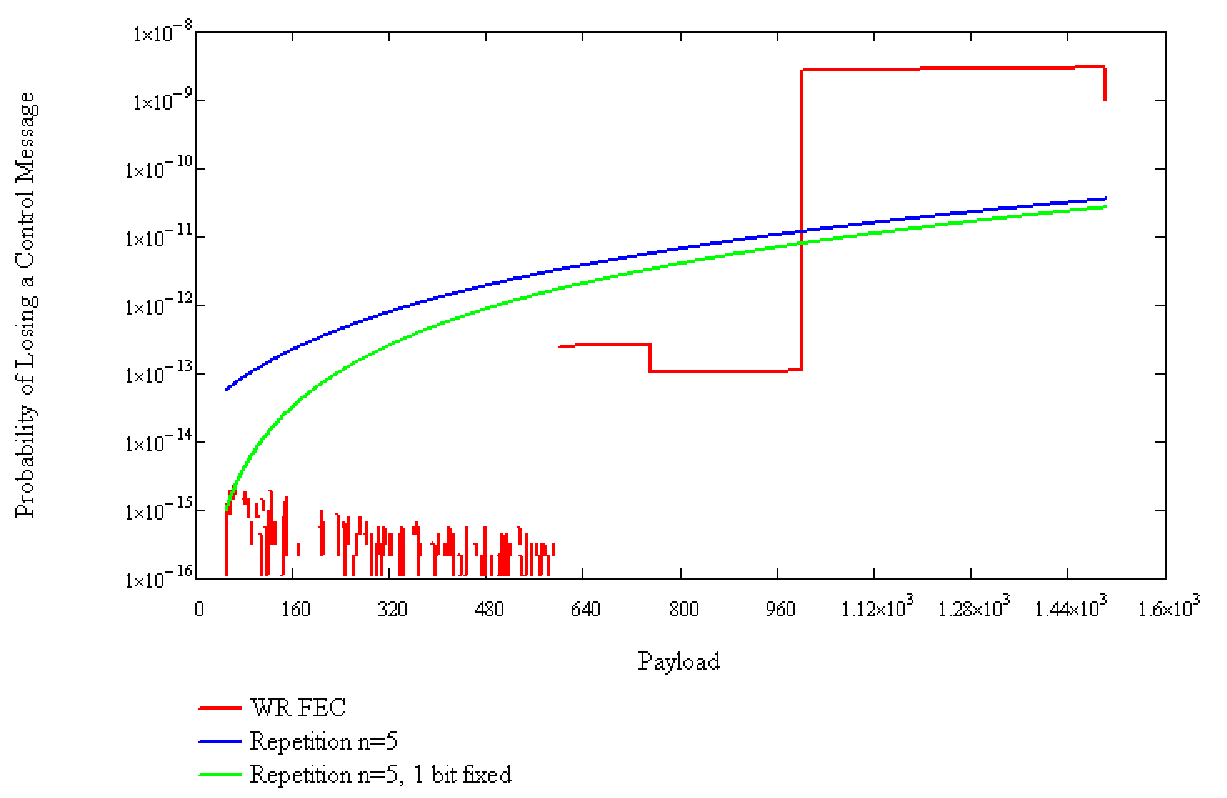
\includegraphics[scale=0.60]{robustness/P_error_control_msg_CERN.ps}
        \captionof{figure}{Probability of Losing a Control Message}
         \label{fig:wrRSTPtopologies}
\end{center}

The Figure ~\ref{fig:wrRSTPtopologies} compares the FEC scheme proposed with a simple repetition code.


\begin{center}
        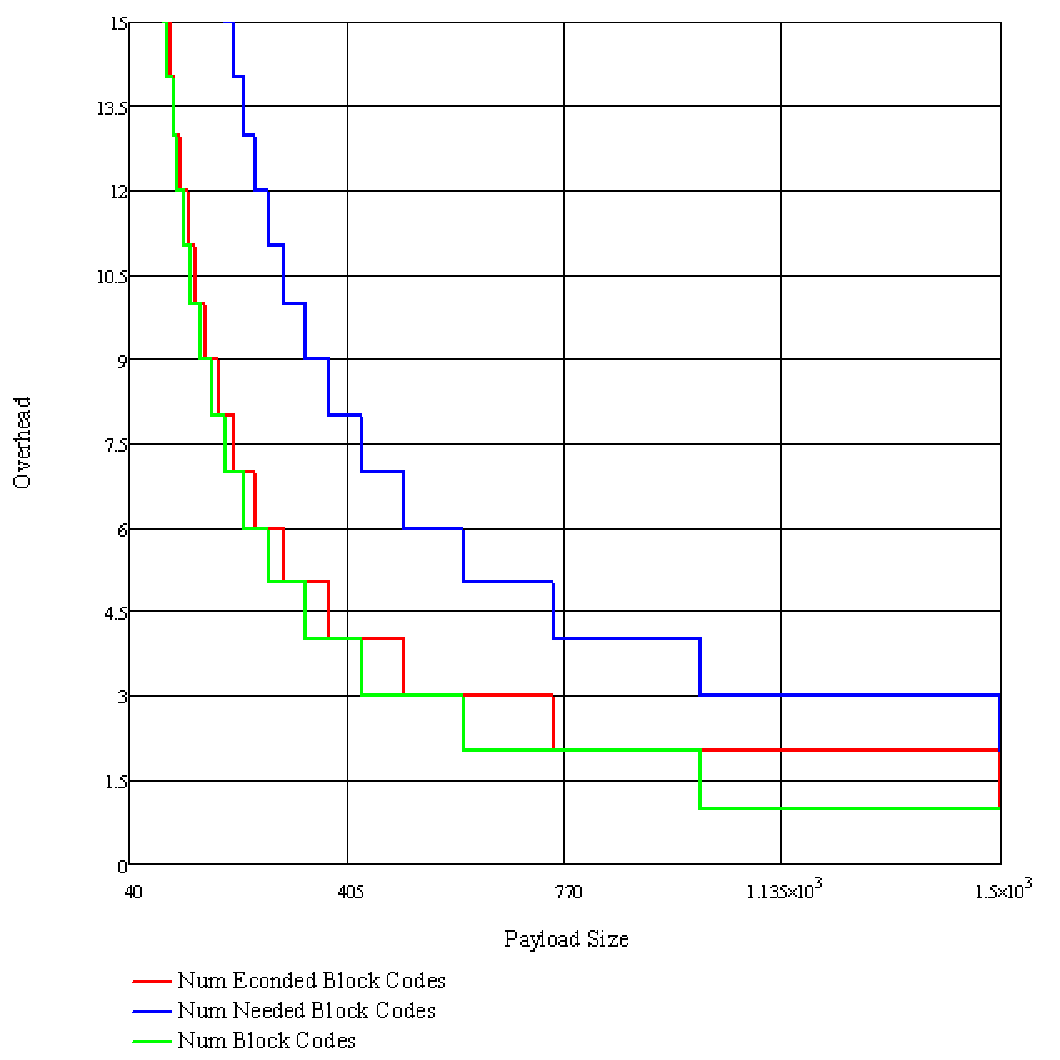
\includegraphics[scale=0.60]{robustness/overhead_cern.ps}
        \captionof{figure}{Overhead introduced by the WR FEC Scheme}
         \label{fig:wrRSTPtopologies}
\end{center}



\subsection{WR FEC Graps in  GSI Network}


\begin{center}
        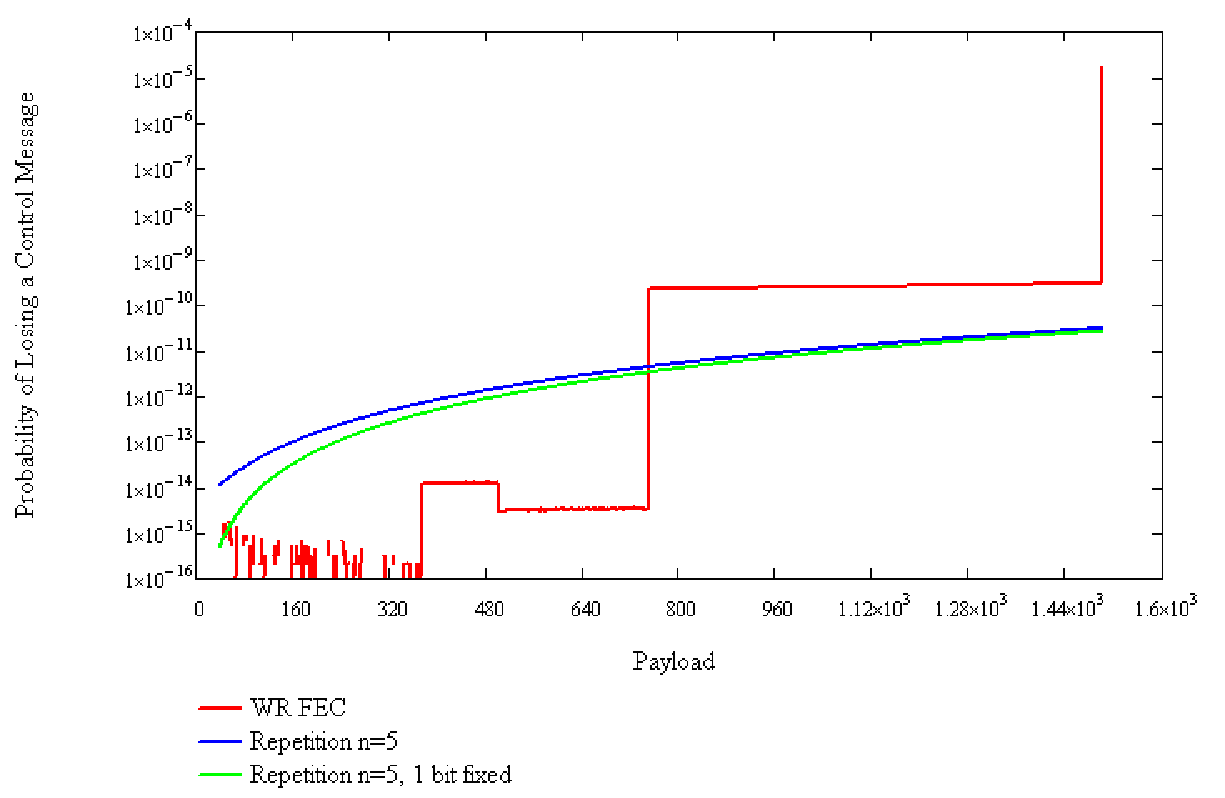
\includegraphics[scale=0.60]{robustness/P_error_control_msg_GSI.ps}
        \captionof{figure}{Probability of Losing a Control Message}
         \label{fig:wrRSTPtopologies}
\end{center}


The Figure ~\ref{fig:wrRSTPtopologies} compares the FEC scheme proposed with a simple repetition code.

\begin{center}
        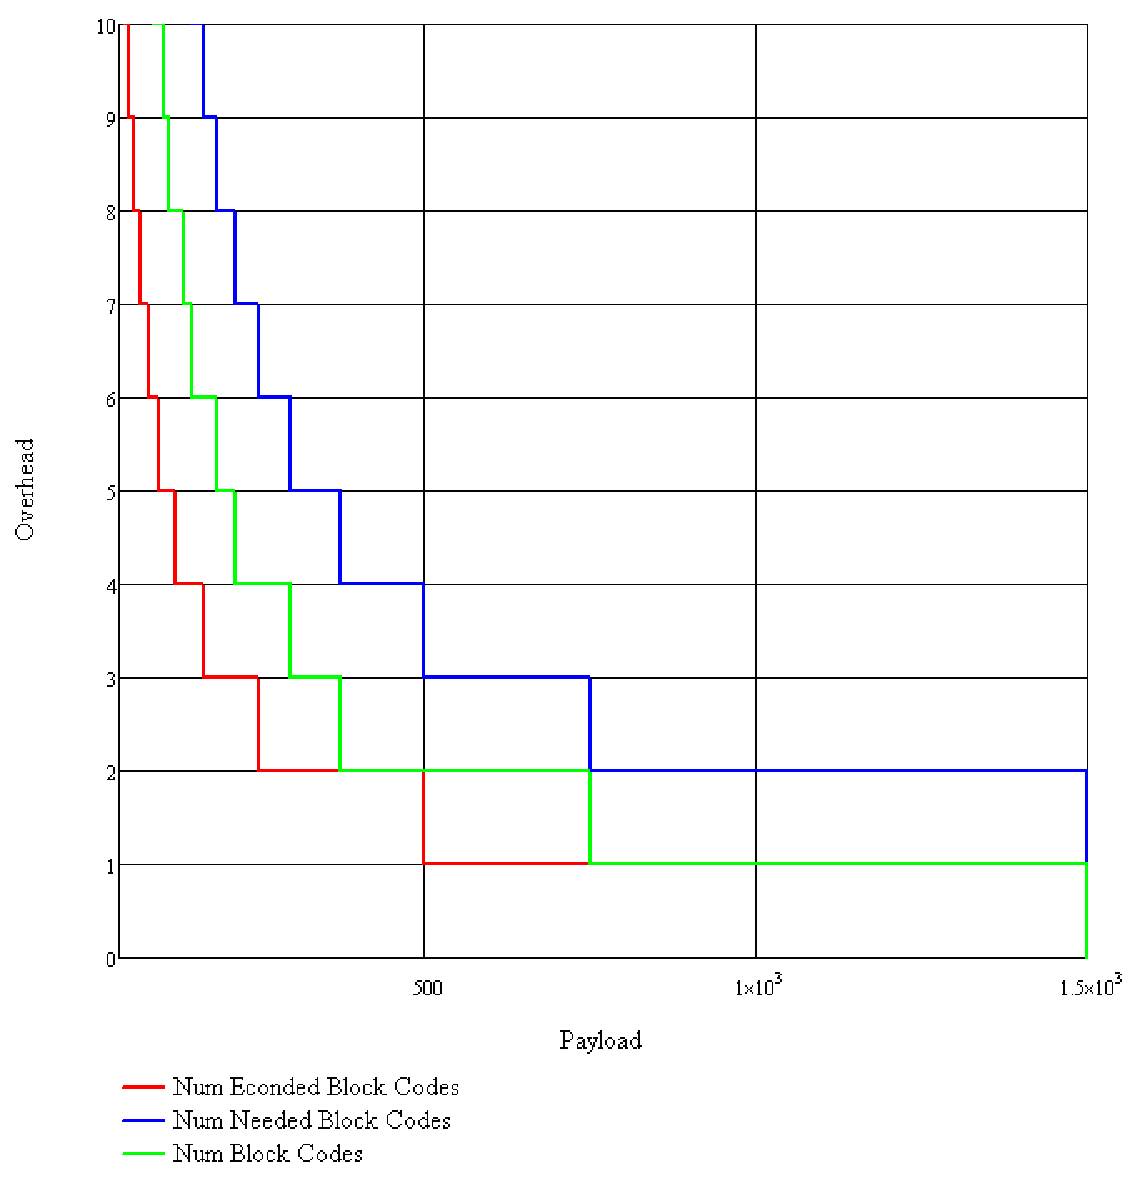
\includegraphics[scale=0.60]{robustness/overhead_gsi.ps}
        \captionof{figure}{Overhead introduced by the WR FEC Scheme}
         \label{fig:wrRSTPtopologies}
\end{center}

\label{app:wr_fec_Graphs}









